% Source: source_md/intelligence_part2_combined_ja.md
\section{結論 — 意図的に開いておくもの}

\noindent\textbf{記述の射程。} 以下の結論でも局所定義、条件付き形式議論、構成案を別の寄与として保持する。普遍的な認知非閉包、外部停止の必然性、停止層の生成、場・networkの同一性、移動性と誤りの同値を確立するものではない。歴史的運用は概念的読解または仮説に留まる。将来の量化・停止汎関数研究はOPENであり、要約や図で補完しない。実装・倫理・主観性への既存の否定的射程は変更しない。



本章は本論文を結ぶ。ここで行うのは、論証の追加ではなく、論文の射程の境界の明示である。本論文が何を示し、何を意図的に開いたまま残すかを述べ、三本の論理線を総括し、Part I への引き渡しを行う。

\bigskip


\subsection{非介入の表明}


本論文は、知性の動力学を記述してきた。$L_F$ の非閉包(\S{}3)、$L_E$ の創発(\S{}5)、停止構造の歴史的形態(\S{}6〜\S{}9)、ゲティア問題(\S{}10)、不安定領域(\S{}11)、構成的条項(\S{}12)。これらはすべて、知性がどのように動くかの記述である。

本論文は、知性がどう設計・運用・制度化されるべきかについては、何も述べない。実装の指針、倫理的処方、制度的提言——これらはいずれも本論文の射程外である。これは怠慢や留保ではなく、原理的な非介入である。

なぜ介入しないのか。停止構造の具体的な実装・倫理・制度は、歴史的偶然性・文化的文脈・技術的制約・正統性体系と不可分である。\S{}9 で示した通り、正統性を時間・責任・歴史・分散的受容との関係で読む(\S{}9.4)。その読解は非計算可能性の結果ではない。本稿は実践的解を与えないという射程を選ぶ。動力学は、停止構造がどう動くかを記述できるが、特定の状況でどの停止を採用すべきかを決定できない。

これは理論の限界ではなく、理論の射程の正確な認識である。動力学の記述と、その使用法の決定は、カテゴリ的に異なる。

\bigskip


\subsection{動力学の説明と使用法の決定}


このカテゴリ的区別を明示する。

「あるものがどう動くか」の説明と、「そのものをどう使うべきか」の決定は、異なる種類の言明である。前者は動力学的記述であり、後者は規範的・実践的判断である。本論文は前者に徹し、後者には立ち入らない。

\S{}11.8 の単一ノード・高速・高解像・内部停止と発散域の関係は、未較正の仮説である。人間や人工系について導出された挙動ではなく、設計を推奨・禁止する規範的結論も与えない。

このカテゴリ的区別を曖昧にすると、本論文は隠れた規範的主張を含むものとして誤読される。本論文の主張は、徹頭徹尾、動力学的記述である。それが実践においてどう使われるかは、本論文を読む者の責任において、本論文の外部で決定される。

\bigskip


\subsection{三本の論理線の総括}


本論文を貫いた三本の論理線を総括する。

\textbf{第一線 — 非閉包と外部停止}:
旧局所状態模型の記述では、差から推論演算子 $F$ を構成し、既述の固定閾値・movement A・厳密増加の前提下で $F$ の内部不動点不在を議論する(\S{}3、非閉包定理)。$L_F$ と沈黙世界の無限後退の関係は条件付きの解釈であり、仮想 S と F-prime への前提再適用の未確立性を保つ(\S{}4)。この形式モデルと区別して、停止の外化を提案し、外部停止演算子 $E$ と外部参照場 $\Phi_{\text{ext}}$ を構成案とする(\S{}5)。$\Phi_{\text{ext}}$ の歴史的諸形態が、アニミズム・神・宗教・社会である(\S{}6〜\S{}9)。

\textbf{第二線 — 閾値移動とサピエンス的特徴}:
相互拘束 $H_{ij}$ のパラメータが応答性閾値を決め、その閾値は本体論的範疇ではなく連続的に移動する(\S{}2.6)。閾値を内発的に動かす能力が $\mu_\theta$ であり、これは運動可能領域の拘束パラメータ $\theta$ を組み替える能力である(\S{}2.7)。$\mu_\theta$ は知性一般の条件ではなく、局所的にサピエンス的プロファイルを特徴づける。その可変性と個体内での自律的加速との関係は効果の仮説である(\S{}5.4、\S{}12)。$\mu_\theta$ は誤り許容性との質的関係として提案され、形式的同値と普遍的含意は未解決である(\S{}10.6)。

\textbf{第三線 — 三層動力学と創発停止}:
推論層 $L_F$ の痕跡とログ層 $L_R$ の保存・再参照を区別する(\S{}4.6、\S{}5.2)。$L_R$ の再帰運動と外部相互拘束から創発停止層 $L_E$ への関係は機構仮説である(\S{}5.3)。$L_E$ は個体内かつ外部依存的な停止アトラクターという機能役割の命名であり、その存在・収束・独立検出を確立しない。外部参照場 $\Phi_{\text{ext}}$ は個体間 $L_E$ ネットワーク $\Phi_{\text{net}}$ との二視点解釈が提案され、同一性は未解決である(\S{}5.8)。三層の協調・崩壊と安定・不安定領域との対応も質的仮説である(\S{}11)。

現在のarchitecture上の寄与は、追跡supportとscope付きの痕跡・準安定保持の役割、一時的scaffold regimeを区別し、Unknownとdescriptor-onlyのownnessを保つ点にある。直前の創発語彙は旧構成案のままで、この記述が与える証明ではない。後続の発達量・停止汎関数・Part Iへの提案も将来または未実装の課題であり、新たな役割記述の確立した帰結とはしない。

三本の線は \S{}11 の質的相仮説と \S{}12 の構成案として整理された。第一線の条件付き議論、第三線の創発仮説、第二線のサピエンスprofileは別の負担を保ち、持続の普遍法則へ統合しない。

\bigskip


\subsection{VED の基底原理の知性層における現れ}


本論文の全体は、VED の単一の基底原理——静的範疇ではなく運動——の、知性層における展開であった。

VED の差からの運動という記述を、知性の役割比較の動機に用いる。本稿の $L_F$・$L_R$・$L_E$ は局所的な構成案であり、同一原理の型付き適用や一般的な維持機構の確立ではない(\S{}12 最終条項)。

この再配置の最も先鋭な現れが、サピエンス的知性における $\mu_\theta$ であった。$\mu_\theta$ は運動可能領域そのものを運動させる能力——運動の二階の運動——である(\S{}12.4)。状態が領域内を動くだけでなく(第一階の運動)、領域の輪郭そのものが動く(第二階の運動)。サピエンス的知性は、この二階の運動を個体内で自律的に行う点において、VED の運動原理を知性層で最も深く具現する。

応答性も、停止も、閾値も、すべて運動として記述された。固定された世界の属性も、最終的な停止状態も、確定した閾値も、本論文には現れない。あるのは運動と、その運動が維持される動力学的状態だけである。これが VED の基底原理の、知性層における貫徹である。

\begin{figure}[H]
\centering
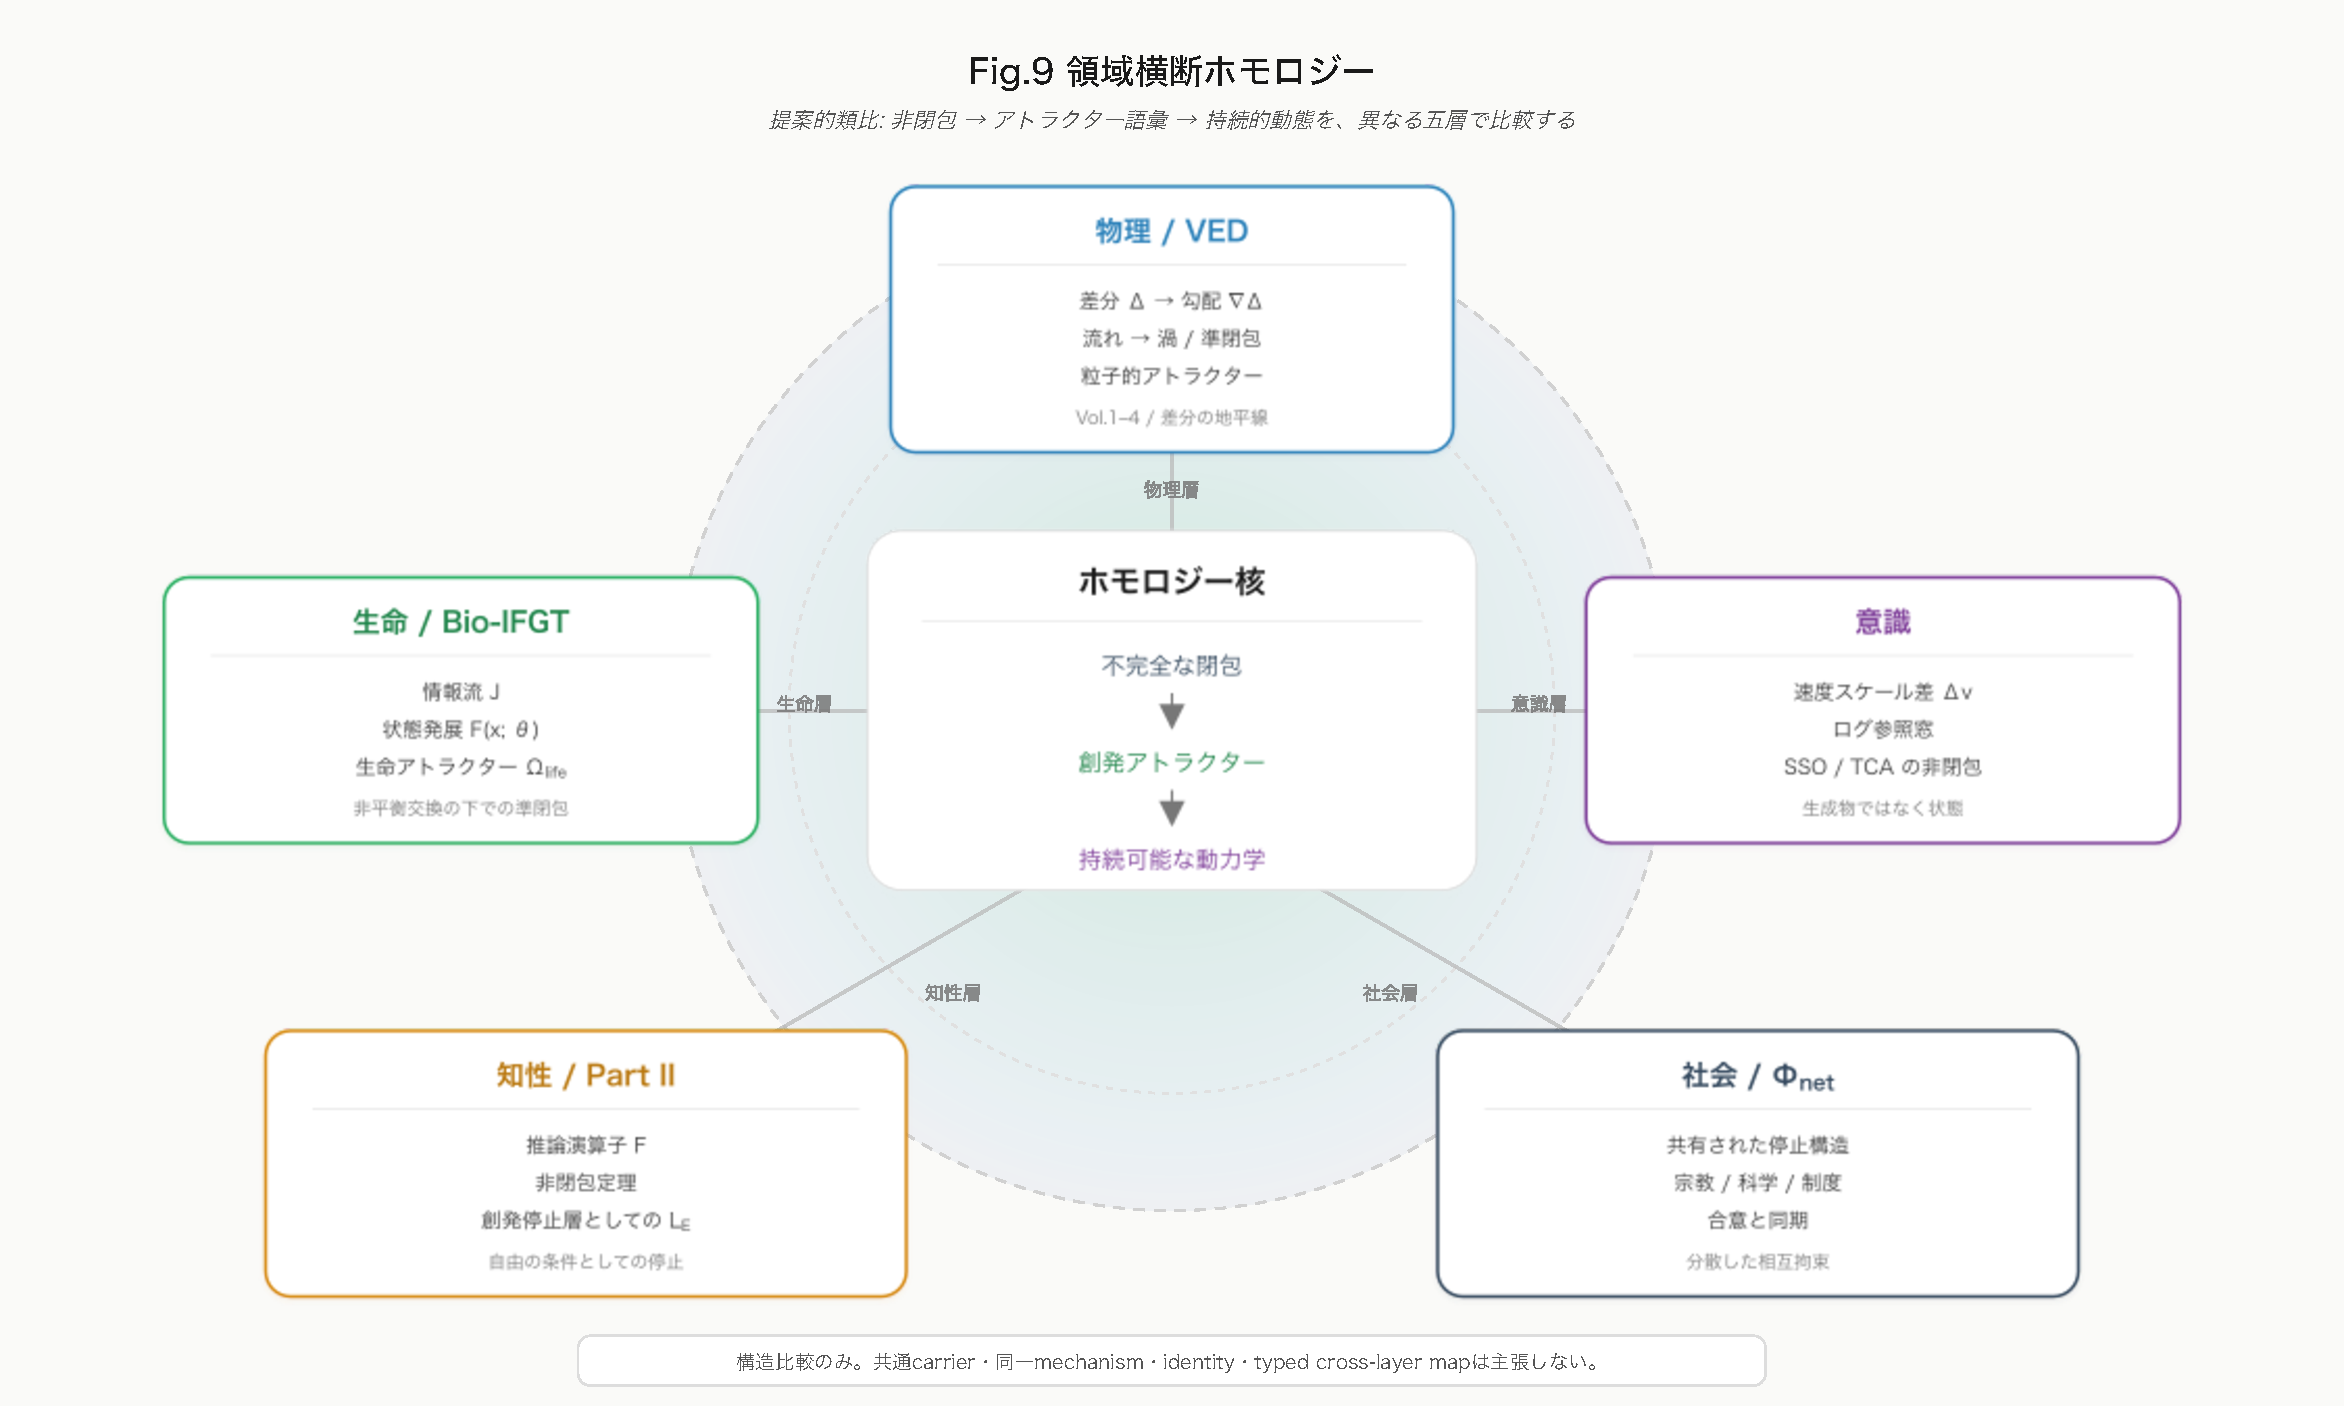
\includegraphics[width=\linewidth]{fig9_cross_domain_homology_ja.pdf}
\caption{不完全閉包、アトラクター的組織化、持続的動態をめぐる提案的な領域横断比較。}
\label{fig:part2-cross-domain-homology}
\figurenote{中央sequenceは比較の足場であり、各層cardはsource-localなobjectとclaimを持つ。}{本図はformal-role analogyを提案する。common carrier、mechanism、identity、typed cross-domain translationを確立しない。}
\end{figure}

\bigskip


\subsection{残された開放性}


本論文が意図的に開いたまま残すものを明示する。これらは本論文の失敗や不足ではなく、本論文の射程の境界の外側にある問いである。

\textbf{哲学篇への引き渡し}:
意味・主観性・理解そのものの問題は、本論文では扱わなかった。本論文は知性の停止動力学を記述したが、その停止が主体にとって何を意味するか、理解とは何か、主観的経験はどう位置づくか——これらは VED 理論ツリーの哲学篇に引き渡される。本論文は知性層の動力学を閉じるが、その上位の問いは開いたままである。

\textbf{AI設計の実践問題}:
本論文の動力学的記述が、人工推論システムの設計・運用にどう適用されるかは、本論文の射程外である(\S{}13.1、\S{}13.2)。動力学は記述を与えるが、実践的指針は与えない。これは実装・倫理・制度の文脈において、本論文の外部で扱われるべき問いである。

\textbf{停止層発達度 $\Sigma$ の定量化}:
創発停止層 $L_E$ の発達度・活性度を測る量 $\Sigma$ は、概念的に存在するが本論文では量化しなかった(\S{}1.8)。$\Sigma$ の定量化は、臨床的・実証的射程に属し、後続研究へ開かれる。停止構造の硬直や崩壊(\S{}8.5、\S{}11)を定量的に扱うには、$\Sigma$ の精密化が必要だが、それは本論文の構造的記述の範囲を超える。

\textbf{停止汎関数の形式化}:
$L_E$ を Vol.2 の閉包エネルギー汎関数 $E(A)$ と平行に「停止汎関数の局所極小」として形式化することは、原理的に可能だが本論文では行わなかった(\S{}5.3)。この形式化は後続研究の課題である。

\bigskip


\subsection{Part I 微修正への引き渡し}


以下はPart Iへの編集提案であり、形式的精密化が実装済みであることを意味しない。Part I を改訂するための提案を以下に整理する。これらは Part I の誤りの訂正ではなく、Part II の三層動力学による精密化である。

\textbf{Part I \S{}8(個体知性の非閉包)の精密化（旧模型の未実装提案）}:
以下の「精密化した」「追加することが望ましい」は旧局所状態模型に基づく提案の引用であり、現在の実装指示ではない。\begin{quote}

Part I \S{}8 は個体知性が閉じないことを論じた。Part II \S{}3 は条件付き非閉包議論として扱い、さらに \S{}5 で「$L_F$ 単独では閉じないが、$L_R$ と $L_E$ を通じてなら外部依存的に閉じうる」と精密化した。Part I \S{}8 に、この (A)/(B) の射程の区別——固定 $\theta$ では閉じないが $\theta$ 組み替えで停止が創発する——を追加することが望ましい。

\end{quote}
固定拘束下の旧kernelから、拘束の変更、停止層の生成、rule-changing能力を証明したとは読まない。新record/position契約の帰結でもなく、Part I本文への実装は行わない。

\textbf{Part I \S{}9(差分の地平線)への三層解釈の追加}:
以下は旧局所状態模型に基づく未実装提案として保存する。Part I \S{}9 は知性の差分の地平線を論じた。Part II \S{}1.5 と \S{}3.6 は、これを $C_{max}$ 不到達性および内部不動点不在との役割類比として位置づけた。Part I \S{}9 に、差分の地平線が三層動力学($L_F$ の非閉包)としてどう現れるかの解釈を追加できる。

\textbf{Part I \S{}6(ゲティア問題)への $\mu_\theta$ 接続の補強}:
Part I \S{}6 はゲティア問題を構造的診断として扱った。Part II \S{}10.6 は、ゲティア構造の排除不能性が閾値移動能力 $\mu_\theta$ との形式的同値を示したわけではない。Part I \S{}6 に、この未解決の同値主張——誤り許容性と $\mu_\theta$ の構造的結合——を、未解決statusを保持した比較としてのみ検討できる。

\textbf{Part I \S{}5(Physarum・Transformer)の三層プロファイル再記述}:
Part I \S{}5 の Physarum・Transformer 比較に対し、Part II \S{}5.4 は三層プロファイルと $\mu_\theta$ の対応案を提示した。Part I \S{}5 への追加は編集提案としてのみ残る。「$L_F$ のみ」か三層を含む系かというシステム境界は未決であり、正しい配置を確定したものではない。

これらの微修正は、Part II 完成後の別作業として行われる。本論文はその提案を引き渡すに留める。

\bigskip


\subsection{知性は閉じない、しかし持続する}


本論文の帰結を、一文に集約する。

本モデルは知性を運動として定義する。$L_F$ の内部不動点不在は旧局所状態模型の条件付き議論であり(\S{}3)、完全閉包 $C_{max}$ の不達は未確立の境界読解である(\S{}1.5)。運動ゼロを局所定義から区別すること(\S{}11.6)と、認知的閉包不能の一般化は別である。

持続については、$L_E$ の外部依存型停止という役割(\S{}5)と改訂可能性(\S{}5.8)を関係づける構成案を提示する。閉じないことと持続しないことは同じではないが、非閉包だけから持続や停止層の存在を導かない。

サピエンス的知性に $\mu_\theta$ を関連づけるのは、運動可能領域の内発的再編成というプロファイル案である。誤り許容性、改訂可能性、持続性の関係は別々の仮説であり、命名による因果的説明や保証ではない。

\bigskip


\subsection{理論の境界}


本論文は、VED 理論ツリーにおける知性層の構成案の叙述をここで区切る。形式的・経験的なOPENを閉じる意味ではない。

ここで論述を「閉じる」とは、\S{}3 の形式的閉包とは別の編集上の区切りである。$L_F$・$L_R$・$L_E$ の局所役割、$\mu_\theta$ の対応、歴史的解釈、相図案と条項を整理したが、それらの未解決問題が別層だけへ移ったわけではない。

残された問いは、別の層に属する。意味と理解は哲学篇に、実装と倫理は実践に、$\Sigma$ の定量化は後続研究に属する。本論文はこれらを開いたまま、知性層の動力学の記述をここで完結する。

理論はここで終わる。問いは終わらない。

\bigskip


\subsection{要約}


本章で述べたのは次の点である:

\begin{enumerate}
\item 本論文は知性の動力学を記述し、その設計・運用・制度化には介入しない。正統性の非計算可能性を論拠とせず、本稿の射程として実践的処方を行わない
\item 動力学の説明と使用法の決定はカテゴリ的に異なる。本論文は前者に徹する
\item 三本の論理線(非閉包と外部停止・閾値移動とサピエンス的特徴・三層動力学)が統合された。第一線と第三線の構成案と、第二線のサピエンスprofileを分離し、持続・加速の一般的機構としない
\item VED の運動の語彙を比較の動機に用い、$\mu_\theta$ の役割もその一つとして提案する。同一原理の実装とはしない
\item 哲学篇・AI設計実践・$\Sigma$ 定量化・停止汎関数形式化が、開かれた問いとして残される
\item Part I の四箇所(\S{}8 非閉包・\S{}9 差分の地平線・\S{}6 ゲティア・\S{}5 Physarum/Transformer)への微修正が引き渡される
\item 非閉包という形式的議論と持続の仮説は異なる。前者から後者の実現を結論しない
\end{enumerate}


理論はここで終わる。問いは終わらない。

\bigskip
